
\documentclass[a4paper,oneside,12pt,titlepage]{article}\usepackage[]{graphicx}\usepackage[]{color}
% maxwidth is the original width if it is less than linewidth
% otherwise use linewidth (to make sure the graphics do not exceed the margin)
\makeatletter
\def\maxwidth{ %
  \ifdim\Gin@nat@width>\linewidth
    \linewidth
  \else
    \Gin@nat@width
  \fi
}
\makeatother

\definecolor{fgcolor}{rgb}{0.345, 0.345, 0.345}
\newcommand{\hlnum}[1]{\textcolor[rgb]{0.686,0.059,0.569}{#1}}%
\newcommand{\hlstr}[1]{\textcolor[rgb]{0.192,0.494,0.8}{#1}}%
\newcommand{\hlcom}[1]{\textcolor[rgb]{0.678,0.584,0.686}{\textit{#1}}}%
\newcommand{\hlopt}[1]{\textcolor[rgb]{0,0,0}{#1}}%
\newcommand{\hlstd}[1]{\textcolor[rgb]{0.345,0.345,0.345}{#1}}%
\newcommand{\hlkwa}[1]{\textcolor[rgb]{0.161,0.373,0.58}{\textbf{#1}}}%
\newcommand{\hlkwb}[1]{\textcolor[rgb]{0.69,0.353,0.396}{#1}}%
\newcommand{\hlkwc}[1]{\textcolor[rgb]{0.333,0.667,0.333}{#1}}%
\newcommand{\hlkwd}[1]{\textcolor[rgb]{0.737,0.353,0.396}{\textbf{#1}}}%
\let\hlipl\hlkwb

\usepackage{framed}
\makeatletter
\newenvironment{kframe}{%
 \def\at@end@of@kframe{}%
 \ifinner\ifhmode%
  \def\at@end@of@kframe{\end{minipage}}%
  \begin{minipage}{\columnwidth}%
 \fi\fi%
 \def\FrameCommand##1{\hskip\@totalleftmargin \hskip-\fboxsep
 \colorbox{shadecolor}{##1}\hskip-\fboxsep
     % There is no \\@totalrightmargin, so:
     \hskip-\linewidth \hskip-\@totalleftmargin \hskip\columnwidth}%
 \MakeFramed {\advance\hsize-\width
   \@totalleftmargin\z@ \linewidth\hsize
   \@setminipage}}%
 {\par\unskip\endMakeFramed%
 \at@end@of@kframe}
\makeatother

\definecolor{shadecolor}{rgb}{.97, .97, .97}
\definecolor{messagecolor}{rgb}{0, 0, 0}
\definecolor{warningcolor}{rgb}{1, 0, 1}
\definecolor{errorcolor}{rgb}{1, 0, 0}
\newenvironment{knitrout}{}{} % an empty environment to be redefined in TeX

\usepackage{alltt}

\usepackage{booktabs}

\usepackage[utf8]{inputenc}
\usepackage[T1]{fontenc}
\usepackage{graphicx}
\usepackage[version=4]{mhchem}
\usepackage[scientific-notation=true]{siunitx}
\usepackage{gensymb}
\usepackage[top=2.5cm, bottom=3cm, left=2.5cm, right=2.5cm]{geometry}
\usepackage{float}
\usepackage{amsmath,amsfonts,amsthm} % Math packages
\title{Preliminary Outlier Detection in Missing Values Free data}
\IfFileExists{upquote.sty}{\usepackage{upquote}}{}
\begin{document}
\maketitle


An initial goal of this work is to provide robust estimates of the composixtion of each rock. This problem is made difficult by the presence of both missing values (laboratories did not measure any composition) and outliers (the measures reported are extreme).

Setting aside the problem of missing values for now, one may look at a subcomposition $\mathbf{x} \in \mathbb{S}^D$ of oxides of major elements.

One begin by importing a dataset, for example GeoPT48, a monzonite.


\begin{knitrout}
\definecolor{shadecolor}{rgb}{0.969, 0.969, 0.969}\color{fgcolor}\begin{kframe}


{\ttfamily\noindent\itshape\color{messagecolor}{\#\# -- Attaching packages --------------------------------------- tidyverse 1.3.1 --}}

{\ttfamily\noindent\itshape\color{messagecolor}{\#\# v ggplot2 3.3.5 \ \ \ \ v purrr \ \ 0.3.4\\\#\# v tibble \ 3.1.5 \ \ \ \ v dplyr \ \ 1.0.7\\\#\# v tidyr \ \ 1.1.4 \ \ \ \ v stringr 1.4.0\\\#\# v readr \ \ 1.4.0 \ \ \ \ v forcats 0.5.1}}

{\ttfamily\noindent\itshape\color{messagecolor}{\#\# -- Conflicts ------------------------------------------ tidyverse\_conflicts() --\\\#\# x dplyr::filter() masks stats::filter()\\\#\# x dplyr::lag() \ \ \ masks stats::lag()}}

{\ttfamily\noindent\itshape\color{messagecolor}{\#\# Registered S3 methods overwritten by 'ggtern':\\\#\# \ \ method \ \ \ \ \ \ \ \ \ \ from \ \ \\\#\# \ \ grid.draw.ggplot ggplot2\\\#\# \ \ plot.ggplot \ \ \ \ \ ggplot2\\\#\# \ \ print.ggplot \ \ \ \ ggplot2}}

{\ttfamily\noindent\itshape\color{messagecolor}{\#\# --\\\#\# Remember to cite, run citation(package = 'ggtern') for further info.\\\#\# --}}

{\ttfamily\noindent\itshape\color{messagecolor}{\#\# \\\#\# Attaching package: 'ggtern'}}

{\ttfamily\noindent\itshape\color{messagecolor}{\#\# The following objects are masked from 'package:ggplot2':\\\#\# \\\#\# \ \ \ \ aes, annotate, ggplot, ggplot\_build, ggplot\_gtable, ggplotGrob,\\\#\# \ \ \ \ ggsave, layer\_data, theme\_bw, theme\_classic, theme\_dark,\\\#\# \ \ \ \ theme\_gray, theme\_light, theme\_linedraw, theme\_minimal, theme\_void}}

{\ttfamily\noindent\itshape\color{messagecolor}{\#\# Welcome to compositions, a package for compositional data analysis.\\\#\# Find an intro with "{}? compositions"{}}}

{\ttfamily\noindent\itshape\color{messagecolor}{\#\# \\\#\# Attaching package: 'compositions'}}

{\ttfamily\noindent\itshape\color{messagecolor}{\#\# The following objects are masked from 'package:stats':\\\#\# \\\#\# \ \ \ \ anova, cor, cov, dist, var}}

{\ttfamily\noindent\itshape\color{messagecolor}{\#\# The following objects are masked from 'package:base':\\\#\# \\\#\# \ \ \ \ \%*\%, norm, scale, scale.default}}

{\ttfamily\noindent\itshape\color{messagecolor}{\#\# Loading required package: pls}}

{\ttfamily\noindent\itshape\color{messagecolor}{\#\# \\\#\# Attaching package: 'pls'}}

{\ttfamily\noindent\itshape\color{messagecolor}{\#\# The following object is masked from 'package:compositions':\\\#\# \\\#\# \ \ \ \ R2}}

{\ttfamily\noindent\itshape\color{messagecolor}{\#\# The following object is masked from 'package:stats':\\\#\# \\\#\# \ \ \ \ loadings}}

{\ttfamily\noindent\itshape\color{messagecolor}{\#\# Loading required package: data.table}}

{\ttfamily\noindent\itshape\color{messagecolor}{\#\# \\\#\# Attaching package: 'data.table'}}

{\ttfamily\noindent\itshape\color{messagecolor}{\#\# The following objects are masked from 'package:dplyr':\\\#\# \\\#\# \ \ \ \ between, first, last}}

{\ttfamily\noindent\itshape\color{messagecolor}{\#\# The following object is masked from 'package:purrr':\\\#\# \\\#\# \ \ \ \ transpose}}

{\ttfamily\noindent\itshape\color{messagecolor}{\#\# Registered S3 method overwritten by 'GGally':\\\#\# \ \ method from \ \ \\\#\# \ \ +.gg \ \ ggplot2}}

{\ttfamily\noindent\itshape\color{messagecolor}{\#\# Registered S3 method overwritten by 'perry':\\\#\# \ \ method \ \ \ \ \ \ \ from \ \ \\\#\# \ \ print.cvFolds cvTools}}

{\ttfamily\noindent\itshape\color{messagecolor}{\#\# \\\#\# Attaching package: 'robCompositions'}}

{\ttfamily\noindent\itshape\color{messagecolor}{\#\# The following object is masked from 'package:compositions':\\\#\# \\\#\# \ \ \ \ variation}}

{\ttfamily\noindent\itshape\color{messagecolor}{\#\# \\\#\# Attaching package: 'robustbase'}}

{\ttfamily\noindent\itshape\color{messagecolor}{\#\# The following object is masked from 'package:robCompositions':\\\#\# \\\#\# \ \ \ \ alcohol}}

{\ttfamily\noindent\itshape\color{messagecolor}{\#\# Scalable Robust Estimators with High Breakdown Point (version 1.5-5)}}\end{kframe}
\end{knitrout}


\begin{knitrout}
\definecolor{shadecolor}{rgb}{0.969, 0.969, 0.969}\color{fgcolor}\begin{kframe}
\begin{alltt}
\hlkwd{setwd}\hlstd{(}\hlstr{"/home/max/Documents/MStatistics/MA2/Thesis/Repository/"}\hlstd{)}
\hlstd{data} \hlkwb{<-} \hlkwd{read_csv}\hlstd{(}\hlstr{"data/raw/GeoPT48 -84Ra.csv"}\hlstd{)}
\end{alltt}


{\ttfamily\noindent\itshape\color{messagecolor}{\#\# \\\#\# -- Column specification --------------------------------------------------------\\\#\# cols(\\\#\# \ \ .default = col\_double(),\\\#\# \ \ Laboratory = col\_character(),\\\#\# \ \ Au = col\_logical(),\\\#\# \ \ N = col\_logical(),\\\#\# \ \ Os = col\_logical()\\\#\# )\\\#\# i Use `spec()` for the full column specifications.}}\end{kframe}
\end{knitrout}
Then, one looks at the subcomposition of major elements :
\begin{knitrout}
\definecolor{shadecolor}{rgb}{0.969, 0.969, 0.969}\color{fgcolor}\begin{kframe}
\begin{alltt}
\hlstd{sel} \hlkwb{<-}\hlkwd{c}\hlstd{(}\hlstr{"SiO2"}\hlstd{,}\hlstr{"TiO2"}\hlstd{,}\hlstr{"Al2O3"}\hlstd{,}\hlstr{"Fe2O3T"}\hlstd{,}\hlstr{"MnO"}\hlstd{,}\hlstr{"MgO"}\hlstd{,}\hlstr{"CaO"}\hlstd{,}\hlstr{"Na2O"}\hlstd{,}
        \hlstr{"K2O"}\hlstd{,}\hlstr{"P2O5"}\hlstd{)}
\hlstd{df.majors} \hlkwb{<-} \hlkwd{select}\hlstd{(data,}\hlkwd{all_of}\hlstd{(sel))}
\hlcom{# closure operation}
\hlstd{df.majors} \hlkwb{<-} \hlkwd{data.frame}\hlstd{(}\hlkwd{clo}\hlstd{(df.majors))}
\end{alltt}
\end{kframe}
\end{knitrout}
Then  missing values are imputed by the column geometric mean
\begin{knitrout}
\definecolor{shadecolor}{rgb}{0.969, 0.969, 0.969}\color{fgcolor}\begin{kframe}
\begin{alltt}
\hlstd{geomean.v} \hlkwb{<-} \hlkwd{sapply}\hlstd{(}\hlkwd{rbind}\hlstd{(df.majors),geomean)}
\hlkwa{for} \hlstd{(i} \hlkwa{in} \hlnum{1}\hlopt{:}\hlkwd{ncol}\hlstd{(df.majors))\{}
  \hlstd{df.majors[,i][}\hlkwd{is.na}\hlstd{(df.majors[,i])]} \hlkwb{<-} \hlstd{geomean.v[i]}
\hlstd{\}}
\end{alltt}
\end{kframe}
\end{knitrout}

\noindent One then transform the dataset using the CLR transformation which is a mapping  $\mathbb{S}^D -> \mathbb{U}^D$ :
\begin{align}
\mathbf{z} = clr(\mathbf{x} = [log(x_1/g(x)),..,log(x_D/g(x))]
\end{align}
Where $\mathbb{U}^D$ is a subspace of $\mathbb{R}^D$ defined as : 
\begin{align*}
U^D = \Big\{[u_1,..,u_D] : \sum_{i=1}^D = 0  \Big\}
\end{align*}

\begin{knitrout}
\definecolor{shadecolor}{rgb}{0.969, 0.969, 0.969}\color{fgcolor}\begin{kframe}
\begin{alltt}
\hlstd{cr.df} \hlkwb{<-} \hlkwd{data.frame}\hlstd{()}
\hlstd{clr.df} \hlkwb{<-} \hlkwd{data.frame}\hlstd{()}
\hlcom{# cr.df, divide each entries in a column by }
\hlcom{# the geometric mean of this column}
\hlstd{cr.df} \hlkwb{<-} \hlkwd{sweep}\hlstd{(df.majors,}\hlkwc{MARGIN} \hlstd{=} \hlnum{2}\hlstd{,}\hlkwc{FUN}\hlstd{=}\hlstr{"/"}\hlstd{,}\hlkwc{STATS} \hlstd{= geomean.v)}
\hlcom{# clr.df is the natural logarithm of cr.df. }
\hlcom{# Now this dataframe contains clr components}
\hlstd{clr.df} \hlkwb{<-} \hlkwd{log}\hlstd{(cr.df)}
\end{alltt}
\end{kframe}
\end{knitrout}
Then principal component analysis is conducted.
Z denotes the mean-centered data matrix X :  
\begin{align*}
z_{ij} = x_{ij} - \mu_j
\end{align*}
Where $\mu_j$ denotes the arithmetic mean of the j-th column. Recall that here using the arithmetic mean is justified because X now lives in a subspace of $\mathbb{R}^D$ which is no longer constrained by the unit sum.

Perform Singular Value Decomposition on clr.df : 
\begin{align}
Z = UDW^T  = (UD)W^T = Z^{*}W^T,Z \in \mathbb{R}^{n\times(d-1)} U \in \mathbb{R}^{n\times p}, D \in \mathbb{R}^{p\times p}, W \in \mathbb{R}^{(d-1)\times p}
\end{align}
$Z^*$ denotes the projection of the mean-centered data matrix on a space of dimension $p$. Hopefully, $Z^*$ contains enough meaningful information about $Z$ while having a much lower number of dimensions. To evaluate how good $Z^*$ approximates $Z$, one looks at the proportion of variance explained by each of the components and more specifically, the cumulative proportion of variance explained by each of the components when these components are ranked from most to less important.



\begin{knitrout}
\definecolor{shadecolor}{rgb}{0.969, 0.969, 0.969}\color{fgcolor}\begin{kframe}
\begin{alltt}
\hlstd{pca.clr} \hlkwb{<-} \hlkwd{prcomp}\hlstd{(clr.df,}\hlkwc{scale} \hlstd{= T,}\hlkwc{rank.} \hlstd{=} \hlkwd{ncol}\hlstd{(clr.df)}\hlopt{-}\hlnum{1} \hlstd{)}
\hlkwd{summary}\hlstd{(pca.clr)}
\end{alltt}
\begin{verbatim}
## Importance of first k=9 (out of 10) components:
##                           PC1    PC2    PC3     PC4     PC5     PC6     PC7
## Standard deviation     2.5272 1.1288 1.0464 0.72257 0.59620 0.48113 0.23209
## Proportion of Variance 0.6387 0.1274 0.1095 0.05221 0.03555 0.02315 0.00539
## Cumulative Proportion  0.6387 0.7661 0.8756 0.92779 0.96334 0.98649 0.99187
##                            PC8     PC9
## Standard deviation     0.18604 0.17566
## Proportion of Variance 0.00346 0.00309
## Cumulative Proportion  0.99533 0.99842
\end{verbatim}
\end{kframe}
\end{knitrout}
The importance of a component, in terms of proportion of variance explained, is directly related to the D matrix whose eigenvalues squared are directly related to the proportion of variance explained through the relationship : 
\begin{align} \label{variancepca}
\lambda_i = d_i^2/(n-1)
\end{align}
Where $d_i$ denotes the i-th diagonal element in the square matrix D of the singular values and n is the number of principal components which is equal to the dimensionality of the original data matrix X.

Now, one looks at the rank-two approximation of Z (as the biplot does) :
\begin{knitrout}
\definecolor{shadecolor}{rgb}{0.969, 0.969, 0.969}\color{fgcolor}\begin{kframe}
\begin{alltt}
\hlcom{# autoplot}
\hlkwd{autoplot}\hlstd{(pca.clr,}\hlkwc{loadings}\hlstd{=T,}\hlkwc{loadings.label}\hlstd{=T)}\hlopt{+}\hlkwd{theme_bw}\hlstd{()}
\end{alltt}
\end{kframe}
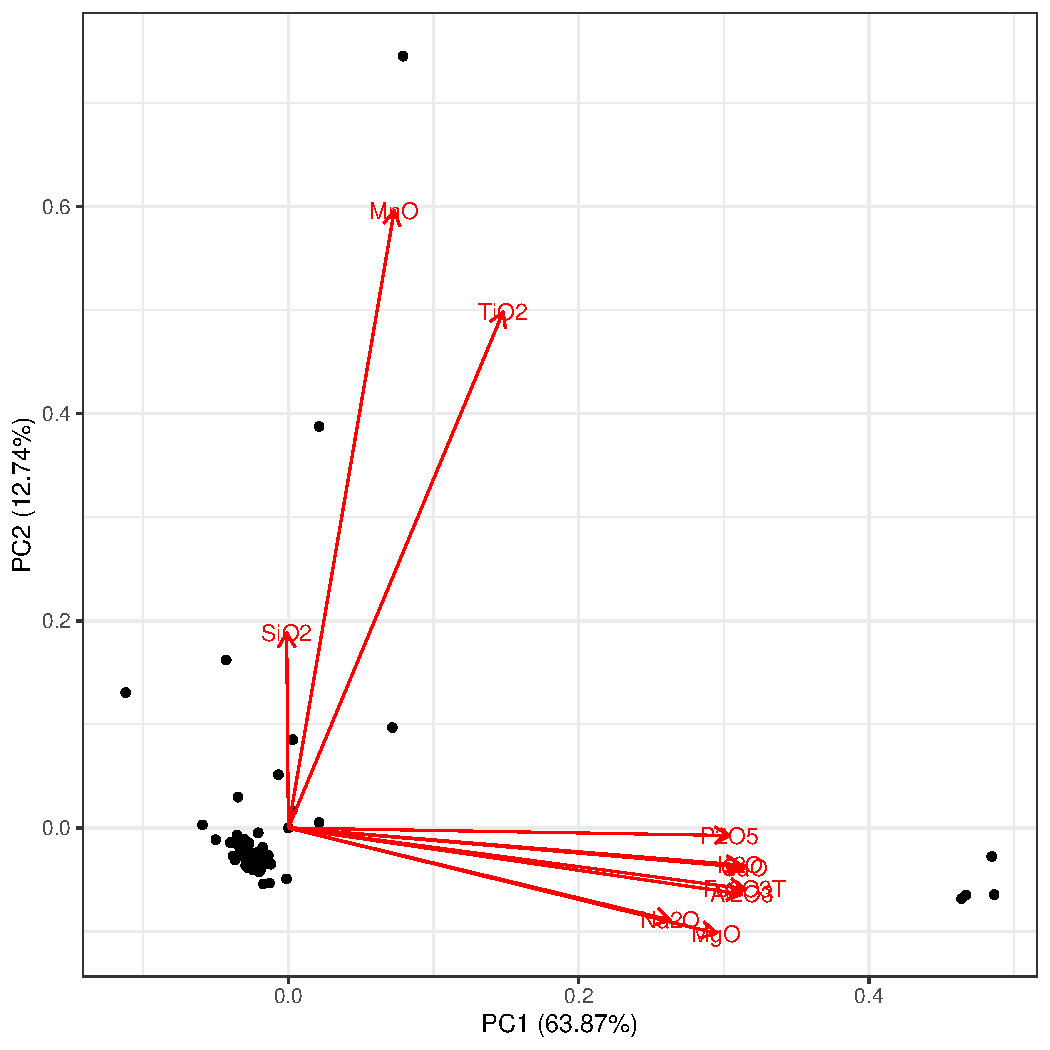
\includegraphics[width=\maxwidth]{figure/unnamed-chunk-7-1} 
\begin{kframe}\begin{alltt}
\hlcom{# manually extracting the rank 2 approximation of Z}
\hlstd{Z.approx} \hlkwb{<-} \hlkwd{data.frame}\hlstd{(pca.clr}\hlopt{$}\hlstd{x[,}\hlkwd{c}\hlstd{(}\hlnum{1}\hlstd{,}\hlnum{2}\hlstd{)])}
\hlkwd{colnames}\hlstd{(Z.approx)} \hlkwb{=} \hlkwd{c}\hlstd{(}\hlstr{"PC1"}\hlstd{,}\hlstr{"PC2"}\hlstd{)}
\hlkwd{ggplot}\hlstd{(}\hlkwd{aes}\hlstd{(}\hlkwc{x}\hlstd{=PC1,}\hlkwc{y}\hlstd{=PC2),}\hlkwc{data}\hlstd{=Z.approx)}\hlopt{+}\hlkwd{theme_bw}\hlstd{()}\hlopt{+}\hlkwd{geom_point}\hlstd{()}
\end{alltt}
\end{kframe}
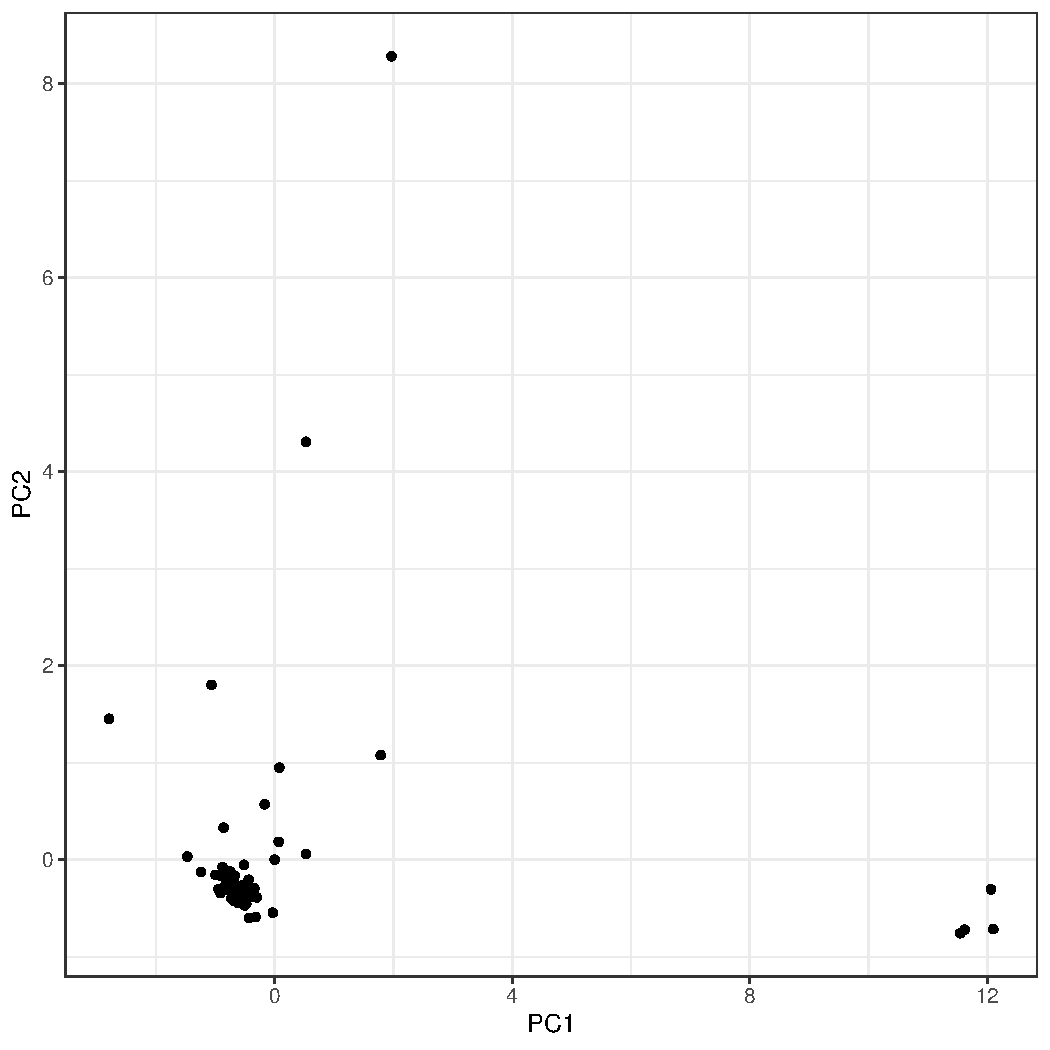
\includegraphics[width=\maxwidth]{figure/unnamed-chunk-7-2} 
\end{knitrout}
Flagging the outliers, remarkable discrepancy between robust method (MCD estimator of the location, MCD is affine equivariant and has a high breakdown value) vs classical method (sample covariance matrix). 
\begin{knitrout}
\definecolor{shadecolor}{rgb}{0.969, 0.969, 0.969}\color{fgcolor}\begin{kframe}
\begin{alltt}
\hlstd{Z2.mcd} \hlkwb{<-} \hlkwd{covMcd}\hlstd{(Z.approx,)}
\hlkwd{tolEllipsePlot}\hlstd{(Z.approx,}\hlkwc{classic} \hlstd{= T)}
\end{alltt}
\end{kframe}
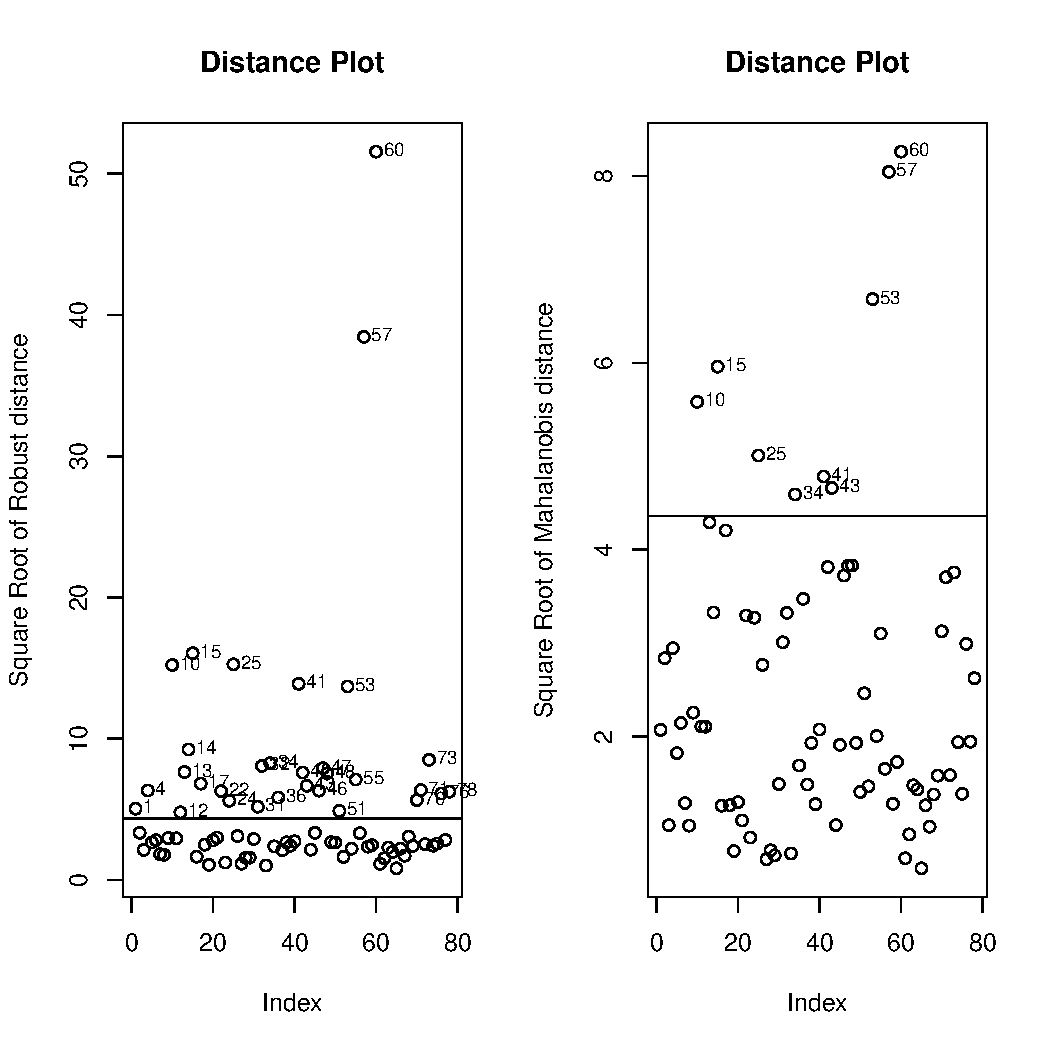
\includegraphics[width=\maxwidth]{figure/unnamed-chunk-8-1} 
\begin{kframe}\begin{alltt}
\hlkwd{plot}\hlstd{(Z2.mcd,}\hlkwc{which} \hlstd{=} \hlkwd{c}\hlstd{(}\hlstr{"distance"}\hlstd{),}\hlkwc{classic} \hlstd{=} \hlnum{TRUE}\hlstd{)}
\end{alltt}
\end{kframe}
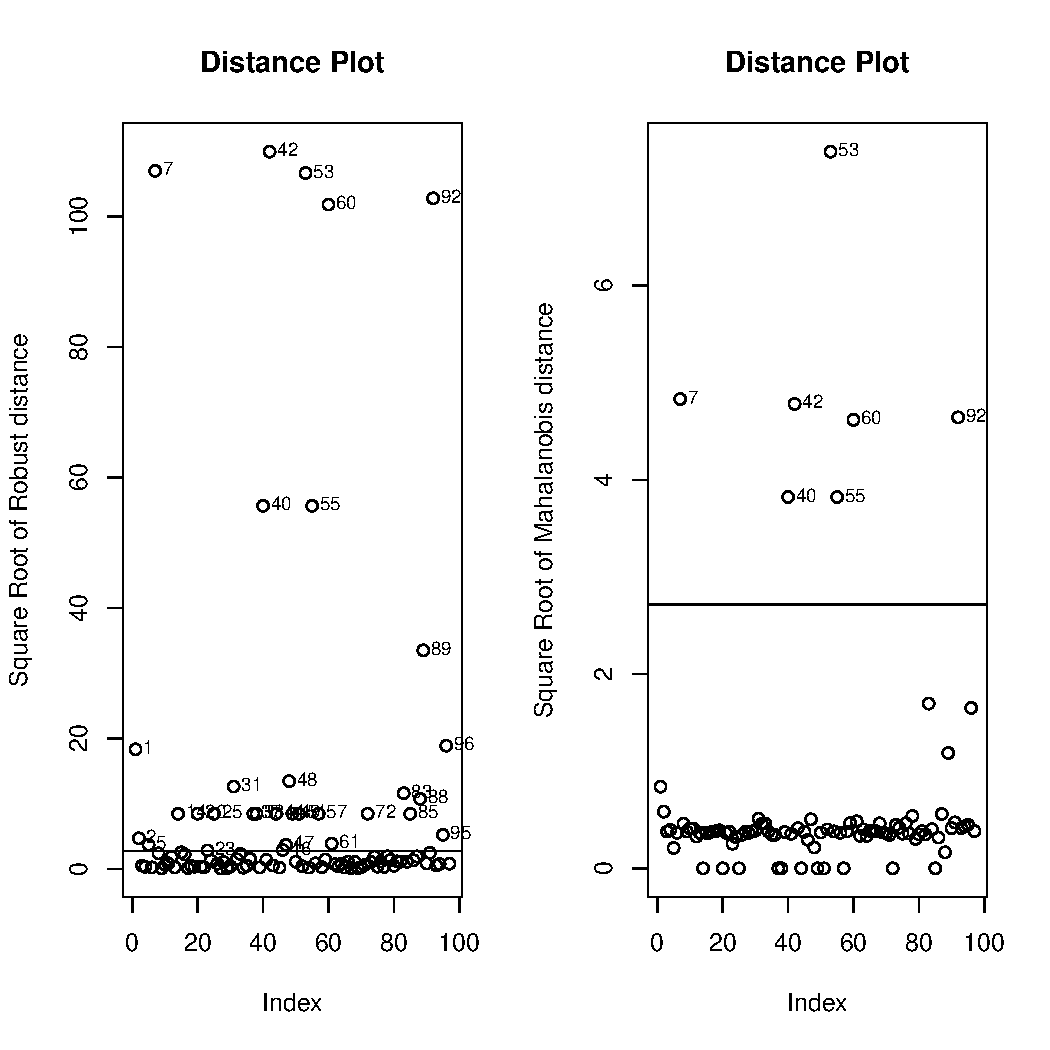
\includegraphics[width=\maxwidth]{figure/unnamed-chunk-8-2} 
\begin{kframe}\begin{alltt}
\hlstd{Z2.outfree} \hlkwb{<-} \hlstd{Z.approx[Z2.mcd}\hlopt{$}\hlstd{best,]}
\hlkwd{ggplot}\hlstd{(}\hlkwd{aes}\hlstd{(}\hlkwc{x}\hlstd{=PC1,}\hlkwc{y}\hlstd{=PC2),}\hlkwc{data}\hlstd{=Z2.outfree)}\hlopt{+}\hlkwd{theme_bw}\hlstd{()}\hlopt{+}\hlkwd{geom_point}\hlstd{()}\hlopt{+}\hlkwd{stat_ellipse}\hlstd{()}
\end{alltt}
\end{kframe}
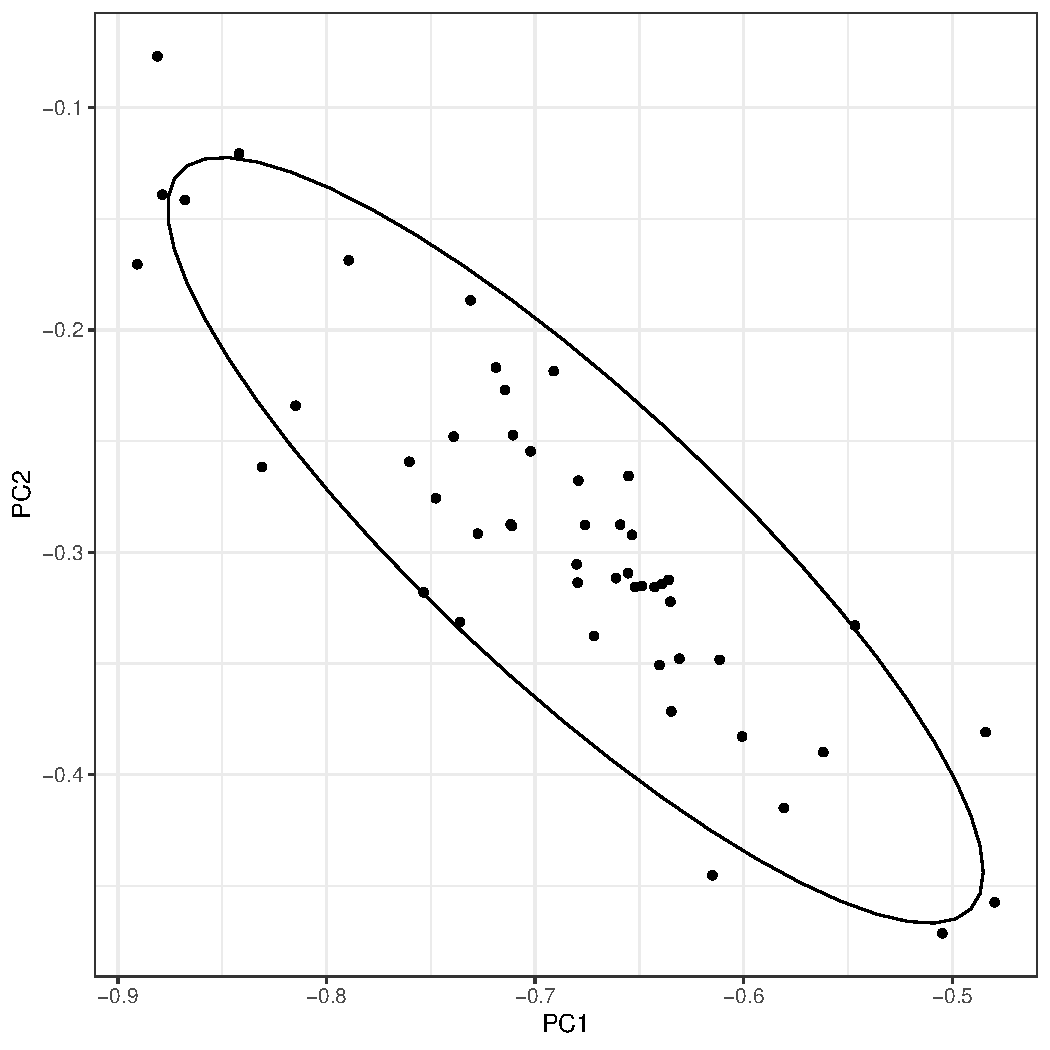
\includegraphics[width=\maxwidth]{figure/unnamed-chunk-8-3} 
\end{knitrout}
This approach has a pitfall. The estimation of the PC is itself not robust. Robcompositions package provides a robust PCA estimation method :
\begin{quote}
The compositional data set is expressed in isometric logratio coordinates. Afterwards, robust principal component analysis is performed. Resulting loadings and scores are back-transformed to the clr space where the compositional biplot can be shown. CITE ROBCOMP R package
\end{quote}
\begin{knitrout}
\definecolor{shadecolor}{rgb}{0.969, 0.969, 0.969}\color{fgcolor}\begin{kframe}
\begin{alltt}
\hlstd{rob.pca.clr} \hlkwb{<-} \hlkwd{pcaCoDa}\hlstd{(df.majors)}
\hlkwd{summary}\hlstd{(rob.pca.clr)}
\end{alltt}
\begin{verbatim}
## Importance of components:
##                           Comp.1     Comp.2     Comp.3     Comp.4     Comp.5
## Standard deviation     0.1314855 0.02931199 0.02737938 0.02224540 0.01728865
## Proportion of Variance 0.8597491 0.04272744 0.03727892 0.02460915 0.01486409
## Cumulative Proportion  0.8597491 0.90247650 0.93975542 0.96436457 0.97922866
##                            Comp.6      Comp.7      Comp.8       Comp.9
## Standard deviation     0.01472258 0.010927871 0.007884733 0.0043980298
## Proportion of Variance 0.01077914 0.005938644 0.003091649 0.0009619057
## Cumulative Proportion  0.99000780 0.995946445 0.999038094 1.0000000000
\end{verbatim}
\end{kframe}
\end{knitrout}
One sees that the first two PC's found by using the robust method explains (89 \%) whereas in the classical method, the first two PC's explained only 76 \%. The outlier detection is repeated in the first 2 robust PC's subspace.
\begin{knitrout}
\definecolor{shadecolor}{rgb}{0.969, 0.969, 0.969}\color{fgcolor}\begin{kframe}
\begin{alltt}
\hlstd{Z.approx.rob} \hlkwb{<-} \hlkwd{data.frame}\hlstd{(rob.pca.clr}\hlopt{$}\hlstd{scores[,}\hlkwd{c}\hlstd{(}\hlnum{1}\hlstd{,}\hlnum{2}\hlstd{)])}
\hlkwd{colnames}\hlstd{(Z.approx.rob)} \hlkwb{=} \hlkwd{c}\hlstd{(}\hlstr{"PC1"}\hlstd{,}\hlstr{"PC2"}\hlstd{)}
\hlkwd{ggplot}\hlstd{(}\hlkwd{aes}\hlstd{(}\hlkwc{x}\hlstd{=PC1,}\hlkwc{y}\hlstd{=PC2),}\hlkwc{data}\hlstd{=Z.approx.rob)}\hlopt{+}\hlkwd{theme_bw}\hlstd{()}\hlopt{+}\hlkwd{geom_point}\hlstd{()}
\end{alltt}
\end{kframe}
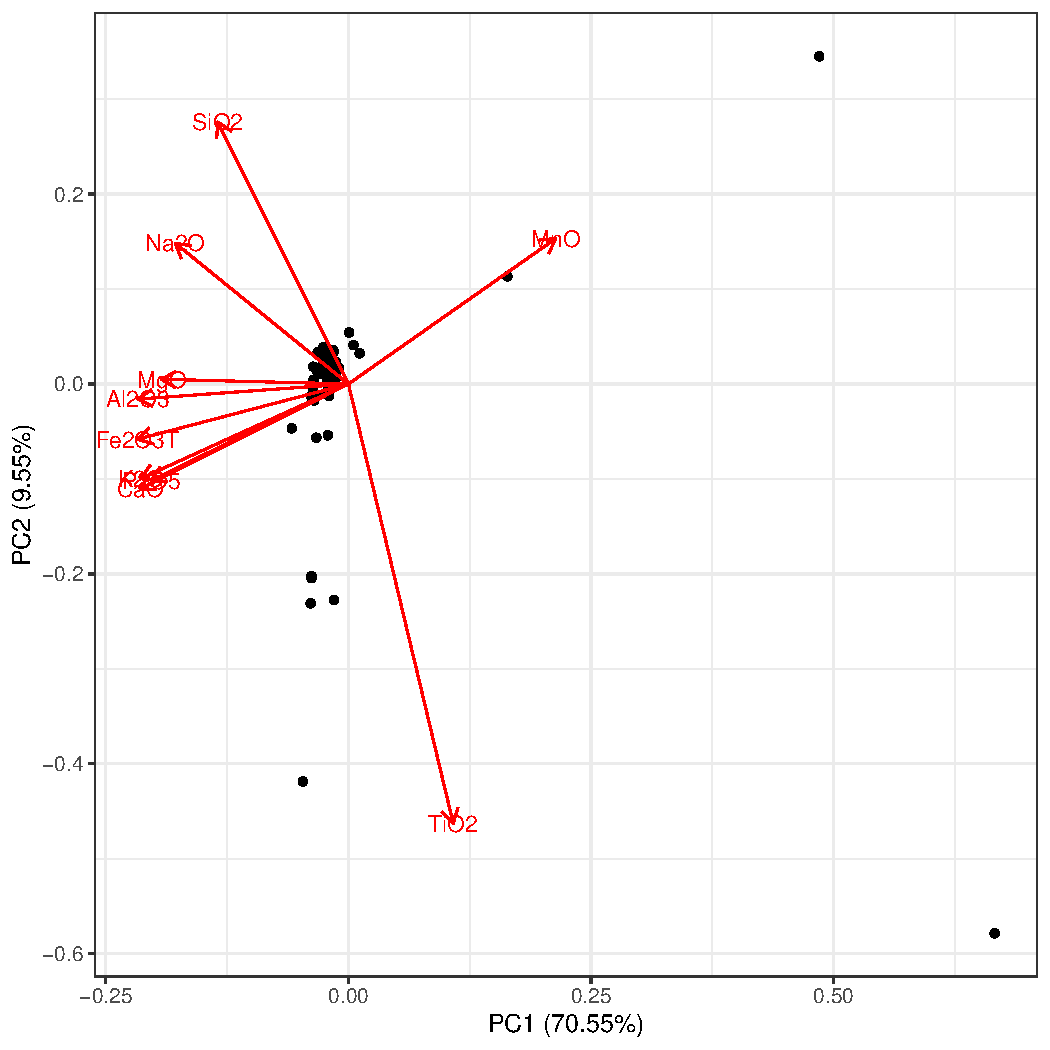
\includegraphics[width=\maxwidth]{figure/unnamed-chunk-10-1} 
\end{knitrout}
At first glance, there seem to be less outliers in the robust first two PC's space. This is checked by using diagnostic plots : 
\begin{knitrout}
\definecolor{shadecolor}{rgb}{0.969, 0.969, 0.969}\color{fgcolor}\begin{kframe}
\begin{alltt}
\hlstd{Z2.rob.mcd} \hlkwb{<-} \hlkwd{covMcd}\hlstd{(Z.approx.rob,)}
\hlkwd{tolEllipsePlot}\hlstd{(Z.approx.rob,}\hlkwc{classic} \hlstd{= T)}
\end{alltt}
\end{kframe}
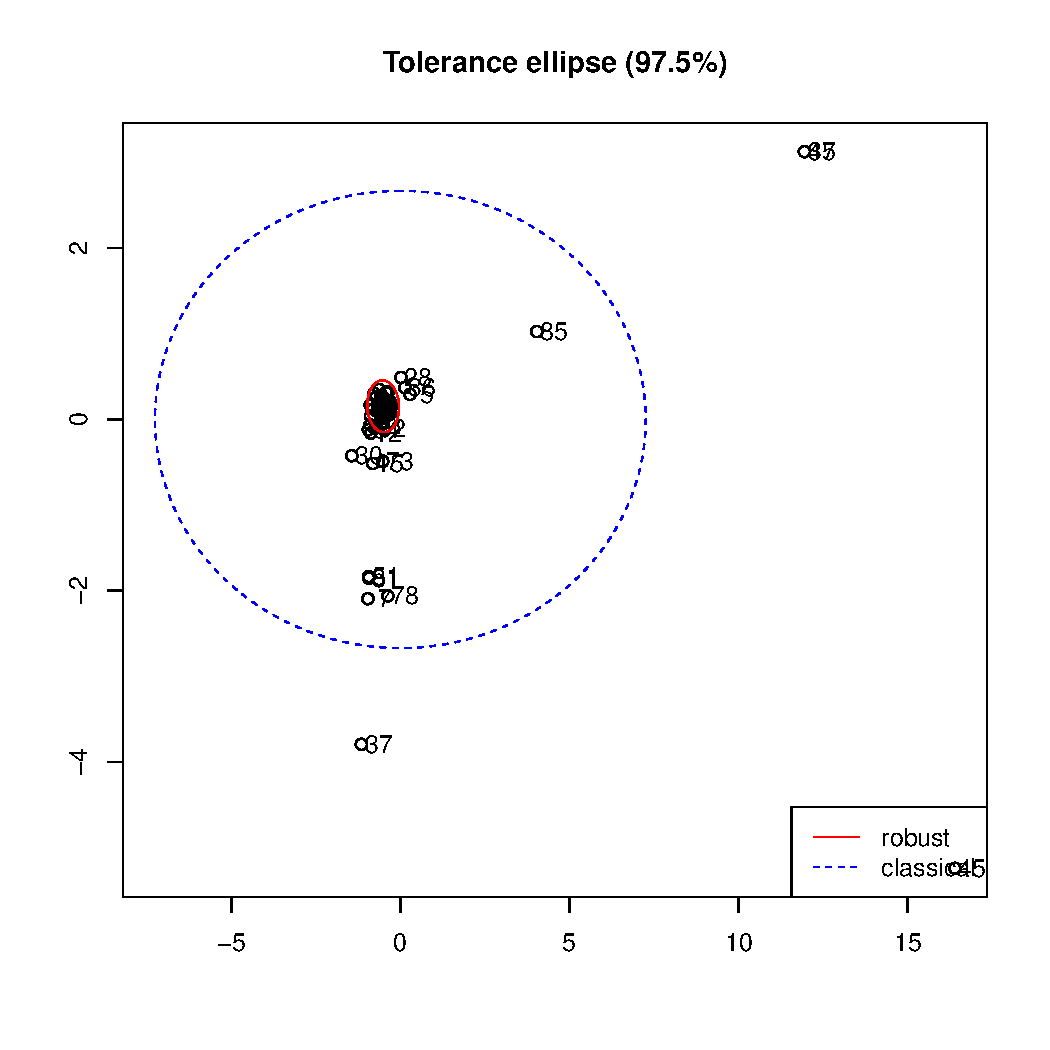
\includegraphics[width=\maxwidth]{figure/unnamed-chunk-11-1} 
\begin{kframe}\begin{alltt}
\hlkwd{plot}\hlstd{(Z2.rob.mcd,}\hlkwc{which} \hlstd{=} \hlkwd{c}\hlstd{(}\hlstr{"distance"}\hlstd{),}\hlkwc{classic} \hlstd{=} \hlnum{TRUE}\hlstd{)}
\end{alltt}
\end{kframe}
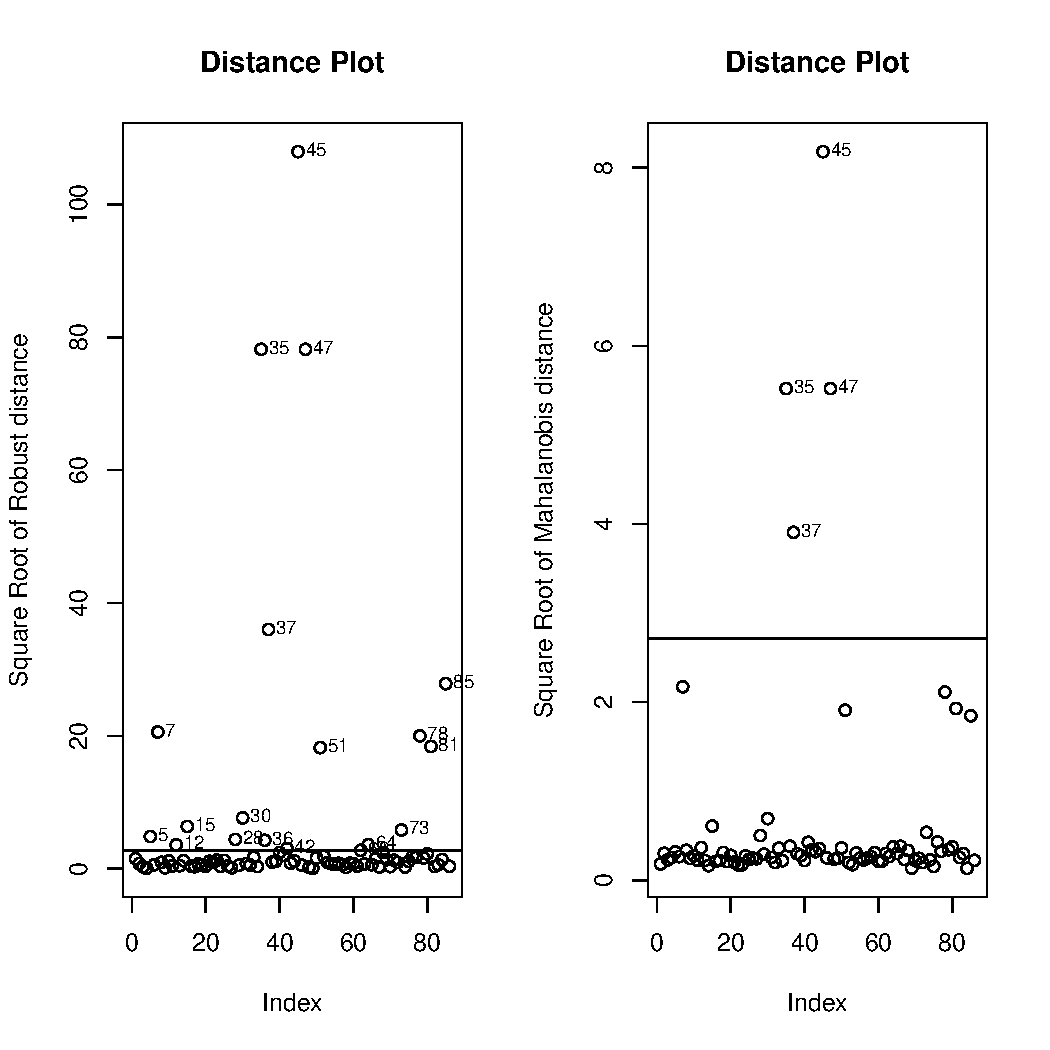
\includegraphics[width=\maxwidth]{figure/unnamed-chunk-11-2} 
\begin{kframe}\begin{alltt}
\hlstd{Z2.rob.outfree} \hlkwb{<-} \hlstd{Z.approx.rob[Z2.rob.mcd}\hlopt{$}\hlstd{best,]}
\hlkwd{ggplot}\hlstd{(}\hlkwd{aes}\hlstd{(}\hlkwc{x}\hlstd{=PC1,}\hlkwc{y}\hlstd{=PC2),}\hlkwc{data}\hlstd{=Z2.rob.outfree)}\hlopt{+}\hlkwd{theme_bw}\hlstd{()}\hlopt{+}\hlkwd{geom_point}\hlstd{()}\hlopt{+}\hlkwd{stat_ellipse}\hlstd{()}
\end{alltt}
\end{kframe}
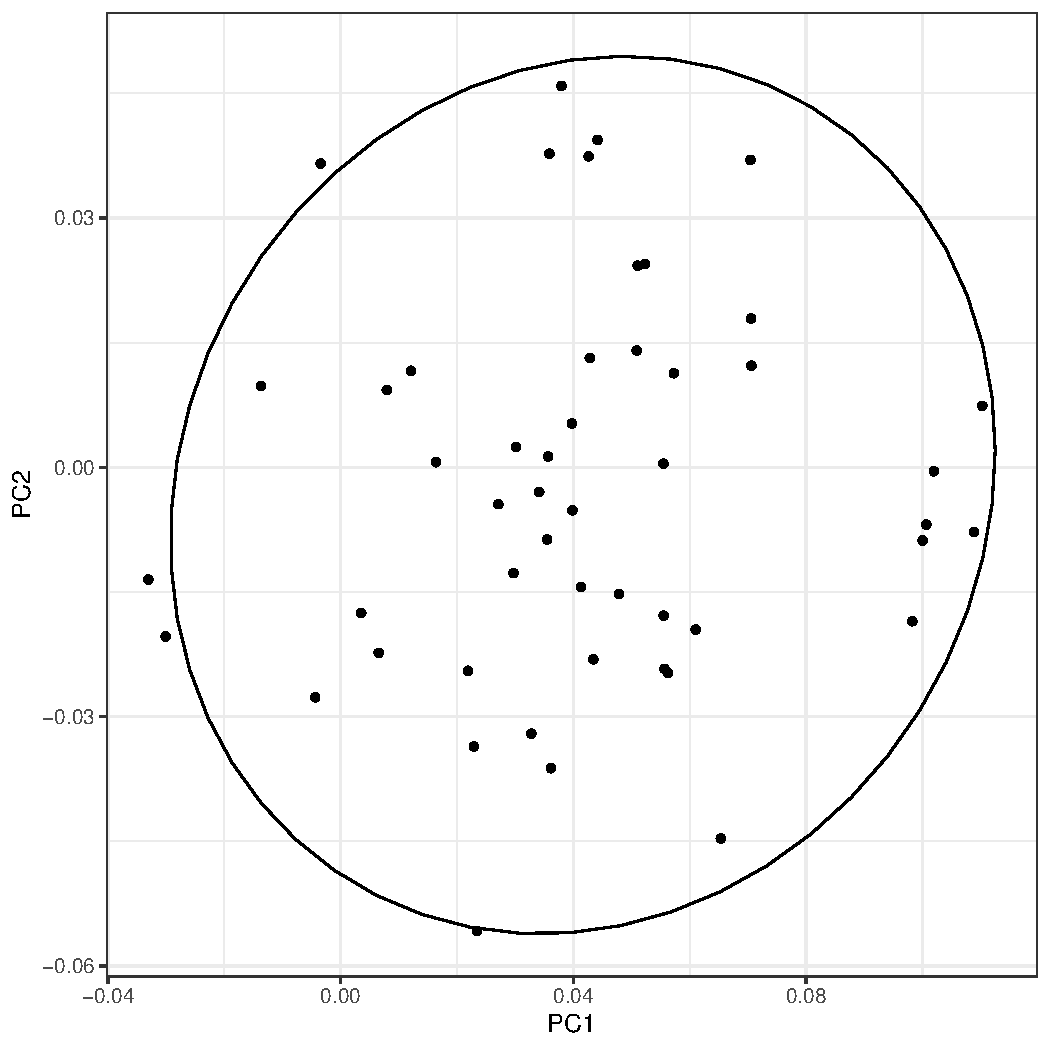
\includegraphics[width=\maxwidth]{figure/unnamed-chunk-11-3} 
\end{knitrout}
There seems to be no association between PC1 and PC2, which makes much more sense. Eventually, an estimation for rock 1 composition is
\begin{knitrout}
\definecolor{shadecolor}{rgb}{0.969, 0.969, 0.969}\color{fgcolor}\begin{kframe}
\begin{alltt}
\hlstd{df.majors.out.free} \hlkwb{<-} \hlstd{df.majors[Z2.rob.mcd}\hlopt{$}\hlstd{best,]}
\hlstd{df.majors.out.free.clr} \hlkwb{<-} \hlkwd{data.frame}\hlstd{(}\hlkwd{clr}\hlstd{(df.majors.out.free))}
\hlstd{clr.mean} \hlkwb{<-} \hlkwd{colMeans}\hlstd{(df.majors.out.free.clr)}
\hlstd{clr.cov} \hlkwb{<-} \hlkwd{Cov}\hlstd{(df.majors.out.free.clr)}

\hlstd{mean.estimate} \hlkwb{<-} \hlkwd{as.vector}\hlstd{(}\hlkwd{clrInv}\hlstd{(clr.mean))}
\hlstd{cov.estimate} \hlkwb{<-} \hlkwd{clrInv}\hlstd{(}\hlkwd{as.matrix}\hlstd{(clr.cov}\hlopt{$}\hlstd{cov))}
\end{alltt}
\end{kframe}
\end{knitrout}
How does it compare with the naive estimates of GeoPT ? 
\begin{knitrout}
\definecolor{shadecolor}{rgb}{0.969, 0.969, 0.969}\color{fgcolor}\begin{kframe}
\begin{alltt}
\hlstd{mean.naive} \hlkwb{<-} \hlkwd{colMeans}\hlstd{(}\hlkwd{clo}\hlstd{(df.majors))}
\hlstd{od} \hlkwb{<-} \hlkwd{outCoDa}\hlstd{(df.majors,} \hlkwc{quantile} \hlstd{=} \hlnum{0.975}\hlstd{,} \hlkwc{method} \hlstd{=} \hlstr{"robust"}\hlstd{,} \hlkwc{alpha} \hlstd{=} \hlnum{0.9}\hlstd{,} \hlkwc{coda} \hlstd{=} \hlnum{TRUE}\hlstd{)}
\hlstd{df.major.wo.outliers} \hlkwb{<-} \hlstd{df.majors[od}\hlopt{$}\hlstd{outlierIndex,]}
\hlstd{mean.naive.wo.outlier} \hlkwb{<-} \hlkwd{colMeans}\hlstd{(}\hlkwd{clo}\hlstd{(df.major.wo.outliers))}
\end{alltt}
\end{kframe}
\end{knitrout}
Not much difference for SiO2 \emph{but} TiO2 concentration is twice as high in the naive way, 5 times higher in the naive way when removing outliers. MnO concentration is 10 times higher in the naive way. 
\begin{knitrout}
\definecolor{shadecolor}{rgb}{0.969, 0.969, 0.969}\color{fgcolor}\begin{kframe}
\begin{alltt}
\hlstd{df} \hlkwb{<-} \hlkwd{data.frame}\hlstd{(mean.estimate,mean.naive,mean.naive.wo.outlier)}
\hlstd{df}
\end{alltt}
\begin{verbatim}
##        mean.estimate  mean.naive mean.naive.wo.outlier
## SiO2     0.581491063 0.563604249           0.512617236
## TiO2     0.010885958 0.015611874           0.029696364
## Al2O3    0.196932296 0.198331406           0.200360748
## Fe2O3T   0.048472449 0.048458236           0.048884754
## MnO      0.001400445 0.012352326           0.045442617
## MgO      0.011369766 0.011289539           0.011110850
## CaO      0.037779434 0.038427579           0.040367724
## Na2O     0.067264543 0.066829195           0.064474391
## K2O      0.038389280 0.038910243           0.040419032
## P2O5     0.006014767 0.006185351           0.006626284
\end{verbatim}
\begin{alltt}
\hlstd{df}\hlopt{$}\hlstd{element} \hlkwb{<-} \hlkwd{row.names}\hlstd{(df)}
\hlstd{df.plot} \hlkwb{<-} \hlstd{df} \hlopt \hlkwd{pivot_longer}\hlstd{(}\hlkwc{cols}\hlstd{=}\hlkwd{starts_with}\hlstd{(}\hlstr{"mean"}\hlstd{))}
\hlstd{df.plot}
\end{alltt}
\begin{verbatim}
## # A tibble: 30 x 3
##    element name                   value
##    <chr>   <chr>                  <dbl>
##  1 SiO2    mean.estimate         0.581 
##  2 SiO2    mean.naive            0.564 
##  3 SiO2    mean.naive.wo.outlier 0.513 
##  4 TiO2    mean.estimate         0.0109
##  5 TiO2    mean.naive            0.0156
##  6 TiO2    mean.naive.wo.outlier 0.0297
##  7 Al2O3   mean.estimate         0.197 
##  8 Al2O3   mean.naive            0.198 
##  9 Al2O3   mean.naive.wo.outlier 0.200 
## 10 Fe2O3T  mean.estimate         0.0485
## # ... with 20 more rows
\end{verbatim}
\begin{alltt}
\hlstd{df.plot}\hlopt{$}\hlstd{group} \hlkwb{<-} \hlkwd{ifelse}\hlstd{(df.plot}\hlopt{$}\hlstd{element} \hlopt \hlkwd{c}\hlstd{(}\hlstr{"SiO2"}\hlstd{,}\hlstr{"Al2O3"}\hlstd{),}\hlkwc{yes} \hlstd{=} \hlstr{"large"}\hlstd{,}\hlstr{"small"}\hlstd{)}
\hlkwd{ggplot}\hlstd{(}\hlkwd{aes}\hlstd{(}\hlkwc{x}\hlstd{=element,}\hlkwc{y}\hlstd{=value),}\hlkwc{data} \hlstd{= df.plot)}\hlopt{+}\hlkwd{geom_col}\hlstd{(}\hlkwd{aes}\hlstd{(}\hlkwc{fill}\hlstd{=name),}\hlkwc{position} \hlstd{=} \hlstr{"dodge"}\hlstd{)}\hlopt{+}\hlkwd{theme_bw}\hlstd{()}\hlopt{+}\hlkwd{facet_grid}\hlstd{(group}\hlopt{~}\hlstd{.,}\hlkwc{scales} \hlstd{=} \hlstr{"free"}\hlstd{)}\hlopt{+}\hlkwd{scale_color_viridis_d}\hlstd{()}
\end{alltt}
\end{kframe}
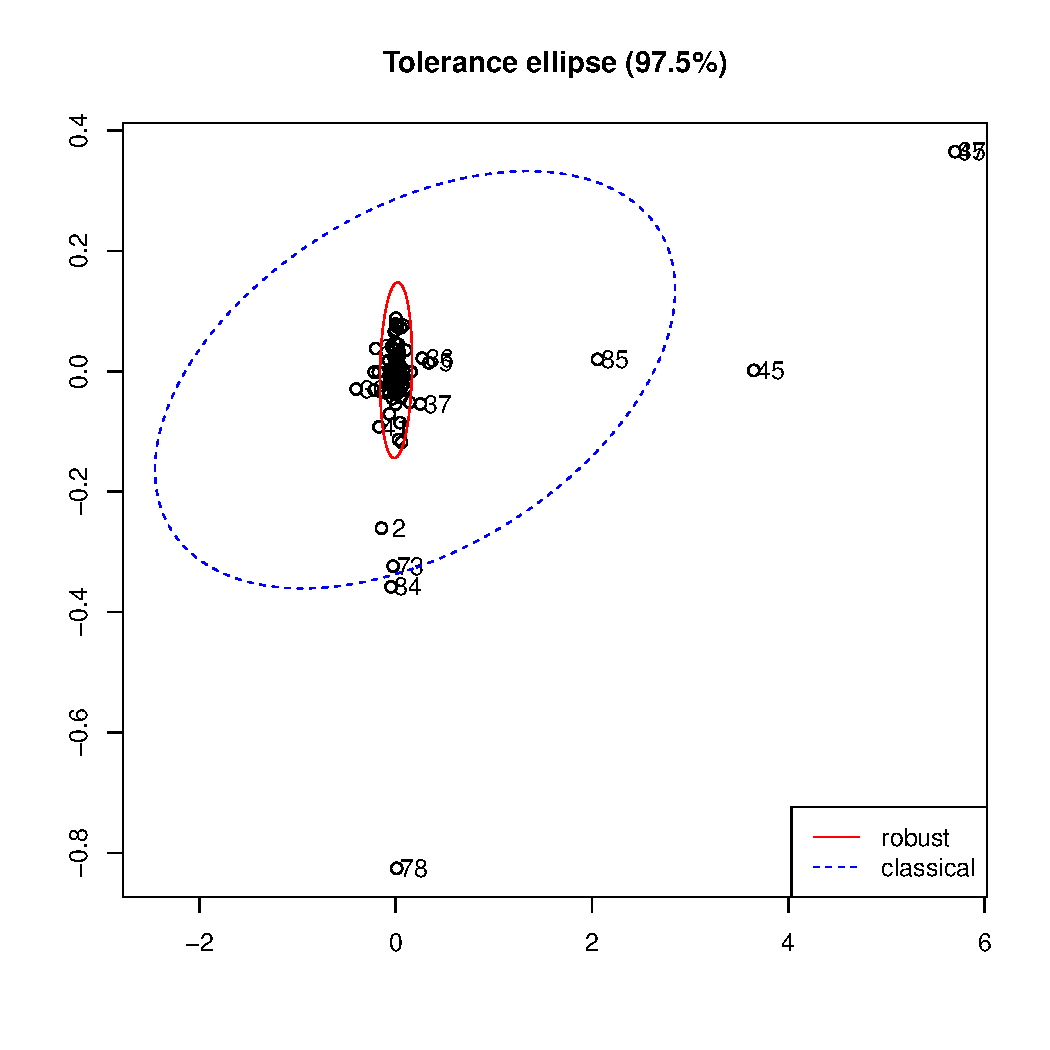
\includegraphics[width=\maxwidth]{figure/unnamed-chunk-14-1} 
\end{knitrout}
Preliminary conclusion : naive without outlier downplay the concentration of elements present in large quantities and blow the concentration of elements present in small quantities.




\end{document}
